\section{1174009 - Dwi Yulianingsih}
\subsection{Parallel Programming Models}
\hfill\break
Model pemrograman paralel ada sebagai abstraksi arsitektur perangkat keras dan memori. Faktanya, model ini tidak spesifik dan tidak merujuk pada jenis mesin atau arsitektur memori tertentu. Mereka dapat diimplementasikan (setidaknya secara teoritis) pada semua jenis mesin. Dibandingkan dengan subdivisi sebelumnya, model pemrograman ini dibuat pada tingkat yang lebih tinggi dan mewakili cara di mana perangkat lunak harus diimplementasikan untuk melakukan perhitungan paralel. Setiap model memiliki caranya sendiri untuk berbagi informasi dengan prosesor lain untuk mengakses memori dan membagi pekerjaan. Secara absolut, tidak ada satu model yang lebih baik dari yang lain. Oleh karena itu, solusi terbaik untuk diterapkan akan sangat tergantung pada masalah yang harus ditangani dan diselesaikan oleh seorang programmer. 
Model yang paling banyak digunakan untuk pemrograman paralel adalah sebagai berikut: 
\begin{itemize}
	\item Model memori bersama 
	\item Model multithread 
	\item Model distribusi memori / pesan terdistribusi
	\item Model paralel data 
\end{itemize}
Dalam resep ini, kami akan memberi Anda gambaran umum tentang model-model ini.
 \begin{figure}[H]
        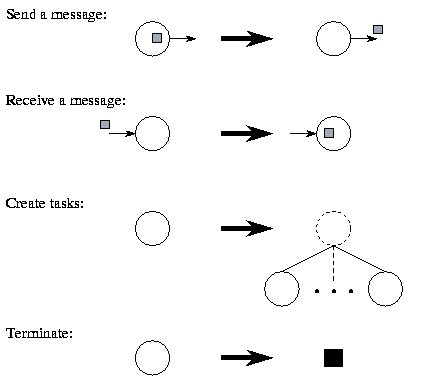
\includegraphics[width=4cm]{figures/kelompok3/1/dwi1.PNG}
        \centering
        \caption{PPM}
\end{figure}
\hfill\break
\subsection{Shared Memory Models}
\hfill\break
Dalam model ini, tugas berbagi area memori tunggal di mana kita dapat membaca dan menulis secara tidak sinkron. Ada mekanisme yang memungkinkan pembuat kode untuk mengontrol akses ke memori bersama; misalnya, mengunci atau semafor. Model ini menawarkan keuntungan bahwa pembuat kode tidak perlu mengklarifikasi komunikasi antar tugas. Kerugian penting, dalam hal kinerja, adalah menjadi lebih sulit untuk memahami dan mengelola lokalitas data. Ini mengacu pada menjaga data tetap lokal untuk prosesor yang bekerja pada menghemat akses memori, penyegaran cache, dan lalu lintas bus yang terjadi ketika beberapa prosesor menggunakan data yang sama.
 \begin{figure}[H]
        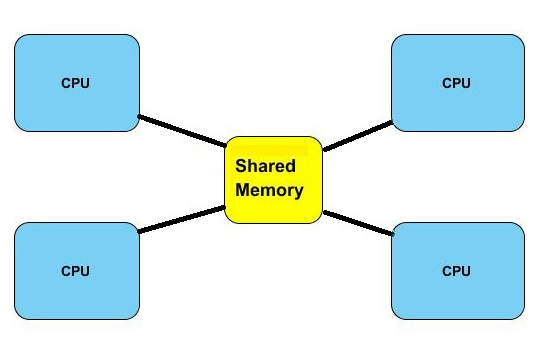
\includegraphics[width=4cm]{figures/kelompok3/1/dwi11.PNG}
        \centering
        \caption{SMM}
\end{figure}
\hfill\break
\subsection{Multithread Models}
\hfill\break
Dalam model ini, suatu proses dapat memiliki beberapa alur eksekusi. Misalnya, bagian berurutan dibuat dan, kemudian, serangkaian tugas dibuat yang dapat dieksekusi secara paralel. Biasanya, model jenis ini digunakan pada arsitektur memori bersama. Jadi, akan sangat penting bagi kita untuk mengelola sinkronisasi antara utas, karena mereka beroperasi pada memori bersama, dan programmer harus mencegah beberapa utas dari memperbarui lokasi yang sama pada saat yang sama. CPU generasi sekarang multithreaded dalam perangkat lunak dan perangkat keras. Utas POSIX (kependekan dari Portable Operating System Interface) adalah contoh klasik dari implementasi multithreading pada perangkat lunak. Teknologi Hyper-Threading Intel mengimplementasikan multithreading pada perangkat keras dengan beralih di antara dua utas saat seseorang terhenti atau menunggu di I / O. Paralelisme dapat dicapai dari model ini, bahkan jika penyelarasan data nonlinier.
 \begin{figure}[H]
        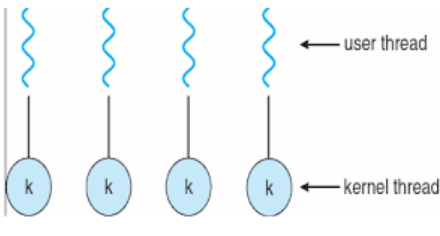
\includegraphics[width=4cm]{figures/kelompok3/1/dwi3.PNG}
        \centering
        \caption{MM}
\end{figure}
\hfill\break
\subsection{Message Passing Models}
\hfill\break
Model pesan lewat biasanya diterapkan dalam kasus di mana setiap prosesor memiliki memori sendiri (sistem memori terdistribusi). Lebih banyak tugas dapat berada di mesin fisik yang sama atau pada jumlah mesin yang sewenang-wenang. Coder bertanggung jawab untuk menentukan paralelisme dan pertukaran data yang terjadi melalui pesan, dan perlu untuk meminta dan memanggil pustaka fungsi dalam kode. Beberapa contoh sudah ada sejak tahun 1980-an, tetapi hanya pada pertengahan 1990-an adalah model standar yang dibuat, mengarah ke standar de facto yang disebut Message Passing Interface (MPI).
 \begin{figure}[H]
        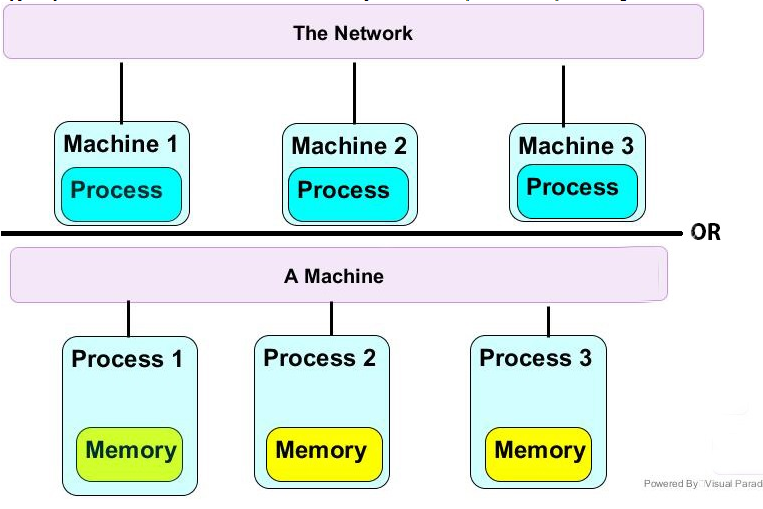
\includegraphics[width=4cm]{figures/kelompok3/1/dwi4.PNG}
        \centering
        \caption{MPM}
\end{figure}


\section{1174008 - Arjun Yuda Firwanda}
\subsection{Komputasi Paralel}
\hfill\break
Pertumbuhan daya komputasi yang disediakan oleh komputer modern telah mengakibatkan kami menghadapi masalah komputasi yang semakin kompleks dalam jangka waktu yang relatif singkat. Sampai awal 2000-an, kompleksitas ditangani dengan meningkatkan jumlah transistor serta frekuensi clock dari sistem prosesor tunggal, yang mencapai puncak 3,5-4 GHz. Namun, peningkatan jumlah transistor menyebabkan peningkatan eksponensial dari daya yang dihabiskan oleh prosesor itu sendiri.

\hfill\break
\subsection{Taksonomi Flynn }
\hfill\break
Taksonomi Flynn adalah sistem untuk mengklasifikasikan arsitektur komputer. Ini didasarkan pada dua konsep utama:
\begin{itemize}
	\item Alur instruksi: Suatu sistem dengan n CPU memiliki n penghitung program dan sesuai dengan penghitung program.
	\item Aliran data: Program yang menghitung fungsi pada daftar data memiliki aliran data.
\end{itemize}
\hfill\break
    \begin{figure}[H]
        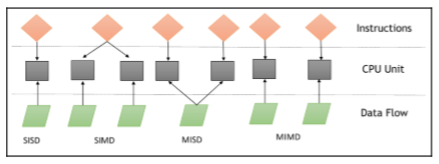
\includegraphics[width=4cm]{figures/kelompok3/1/arjun1.png}
        \centering
        \caption{tf}
    \end{figure}
Ada empat kategori mesin paralel: Instruksi Tunggal, Data Tunggal (SISD), Data Instruksi Berganda (SIMD), Instruksi Berganda Data Tunggal (MISD), dan Data Instruksi Berganda Banyak (MIMD).


\subsection{Single Instruction Single Data}
\hfill\break
Single Instruction Single Data (SISD) Sistem komputasi SISD seperti mesin von Neumann, yang merupakan mesin uniprocessor. 
Dalam siklus clock, CPU menjalankan operasi berikut:
\begin{itemize}
	\item Fetch: CPU mengambil data dan instruksi dari area memori, yang disebut register.
	\item Decode: CPU menerjemahkan instruksi.
	\item Execute: Instruksi dilakukan pada data. Hasil operasi disimpan dalam register lain.
\end{itemize}
\hfill\break
    \begin{figure}[H]
        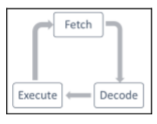
\includegraphics[width=4cm]{figures/kelompok3/1/arjun2.png}
        \centering
        \caption{sisd}
    \end{figure}
\hfill\break
Elemen utama dari arsitektur ini (yaitu, arsitektur von Neumann) adalah sebagai berikut:
\begin{itemize}
	\item Unit memori pusat: Ini digunakan untuk menyimpan instruksi dan data program.
	\item CPU: Ini digunakan untuk mendapatkan instruksi dan / atau data dari unit memori, yang menerjemahkan instruksi dan secara berurutan mengimplementasikannya.
	\item Sistem I atau  O: Ini mengacu pada data input dan output dari program..
\end{itemize}

\section{1174027 - Harun Ar - Rasyid}
\subsection{Introducing Python}
\hfill\break
Python adalah bahasa pemrograman yang kuat, dinamis, dan digunakan dalam berbagai macam aplikasi. \\
Beberapa fitur-fiturnya adalah sebagai berikut:
\begin{itemize}
    \item Sintaks yang mudah dibaca dan jelas.
    \item Perpustakaan standar yang sangat luas.
    \item Pengembangan Cepat dan debugging yang mudah dipelajari.
\end{itemize}
\subsection{Help Function}
\hfill\break
Python interpreter sudah menyediakan sistem bantuan yang valid.
\begin{enumerate}
    \item Help(object)
    \lstinputlisting[firstline=7, lastline=8]{src/kelompok3/1/1.py}
    \begin{figure}[H]
        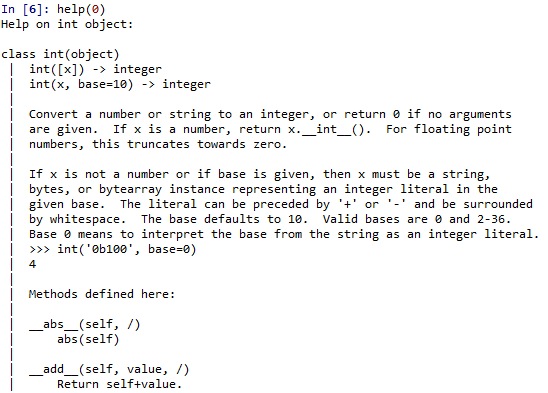
\includegraphics[width=4cm]{figures/kelompok3/1/1.png}
        \centering
        \caption{Hasil Dari Help bagian 1}
    \end{figure}
    \begin{figure}[H]
        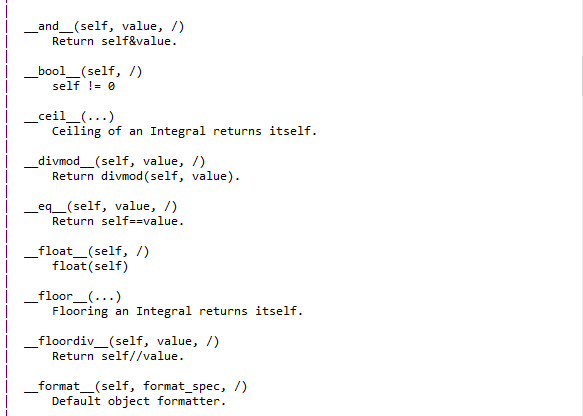
\includegraphics[width=4cm]{figures/kelompok3/1/2.png}
        \centering
        \caption{Hasil Dari Help bagian 2}
    \end{figure}
    \begin{figure}[H]
        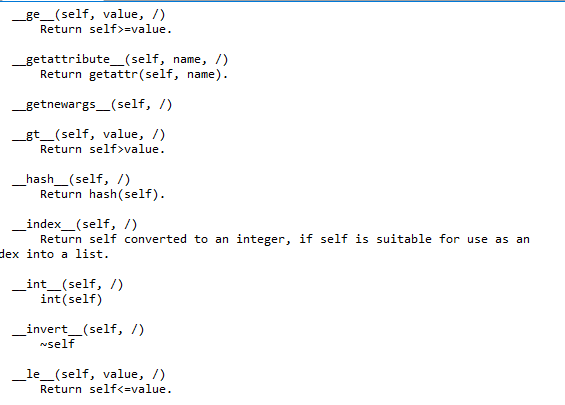
\includegraphics[width=4cm]{figures/kelompok3/1/3.png}
        \centering
        \caption{Hasil Dari Help bagian 3}
    \end{figure}
    \begin{figure}[H]
        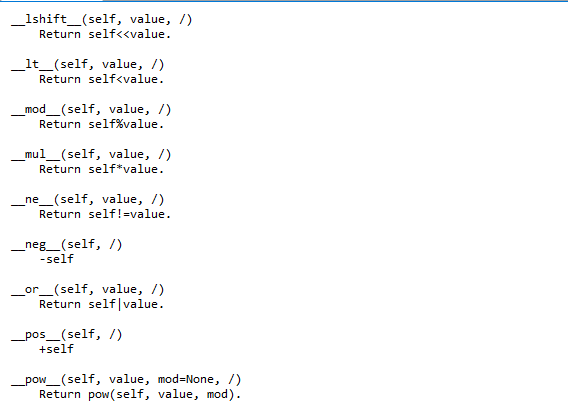
\includegraphics[width=4cm]{figures/kelompok3/1/4.png}
        \centering
        \caption{Hasil Dari Help bagian 4}
    \end{figure}
    \begin{figure}[H]
        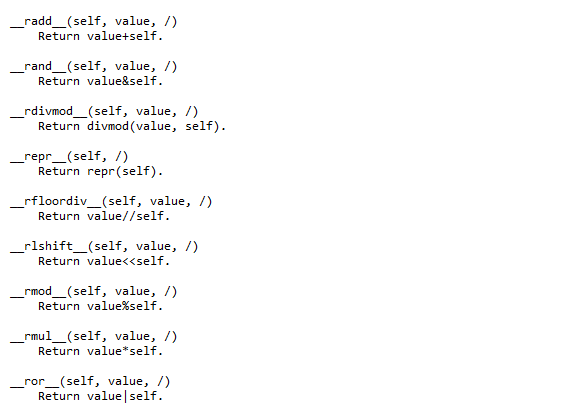
\includegraphics[width=4cm]{figures/kelompok3/1/5.png}
        \centering
        \caption{Hasil Dari Help bagian 5}
    \end{figure}
    \begin{figure}[H]
        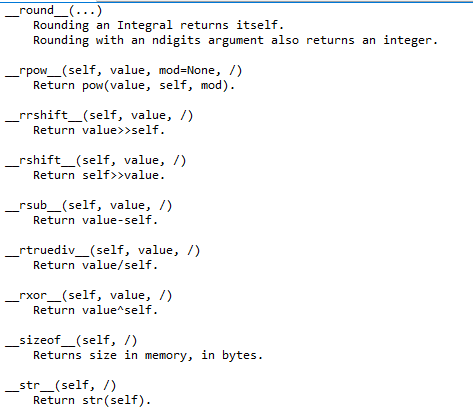
\includegraphics[width=4cm]{figures/kelompok3/1/6.png}
        \centering
        \caption{Hasil Dari Help bagian 6}
    \end{figure}
    \begin{figure}[H]
        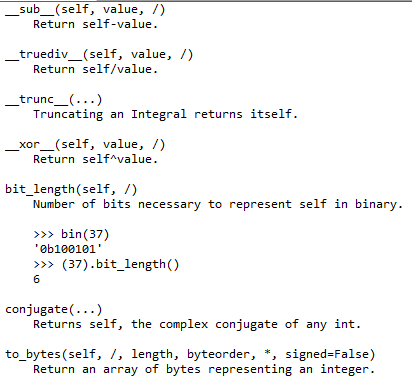
\includegraphics[width=4cm]{figures/kelompok3/1/7.png}
        \centering
        \caption{Hasil Dari Help bagian 7}
    \end{figure}
    \begin{figure}[H]
        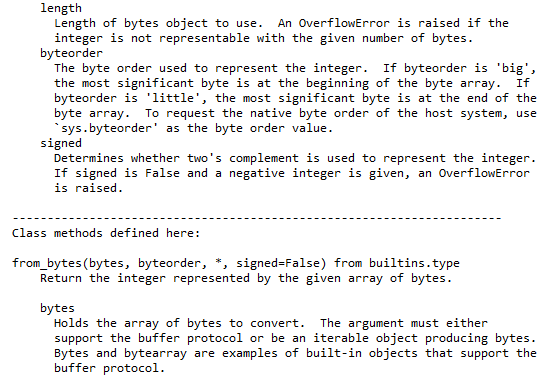
\includegraphics[width=4cm]{figures/kelompok3/1/8.png}
        \centering
        \caption{Hasil Dari Help bagian 8}
    \end{figure}
    \begin{figure}[H]
        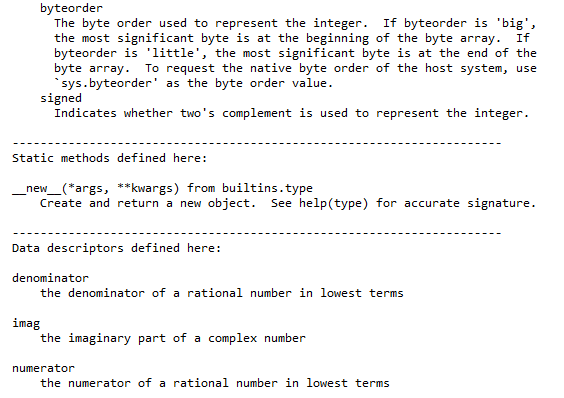
\includegraphics[width=4cm]{figures/kelompok3/1/9.png}
        \centering
        \caption{Hasil Dari Help bagian 9}
    \end{figure}
    \begin{figure}[H]
        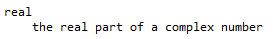
\includegraphics[width=4cm]{figures/kelompok3/1/10.png}
        \centering
        \caption{Hasil Dari Help bagian 10}
    \end{figure}
    \item dir(object)
    \lstinputlisting[firstline=9, lastline=10]{src/kelompok3/1/1.py}
    \begin{figure}[H]
        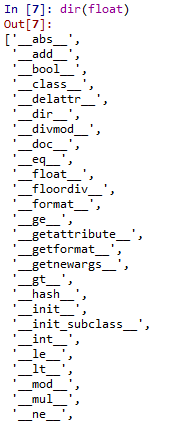
\includegraphics[width=4cm]{figures/kelompok3/1/11.png}
        \centering
        \caption{Hasil Dari Dir Bagian 1}
    \end{figure}
    \begin{figure}[H]
        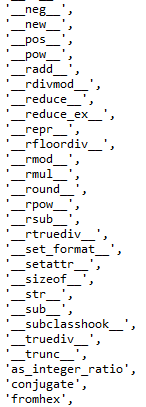
\includegraphics[width=4cm]{figures/kelompok3/1/12.png}
        \centering
        \caption{Hasil Dari Dir Bagian 2}
    \end{figure}
    \begin{figure}[H]
        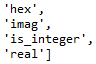
\includegraphics[width=4cm]{figures/kelompok3/1/13.png}
        \centering
        \caption{Hasil Dari Dir Bagian 3}
    \end{figure}
    \item abs document
    \lstinputlisting[firstline=11, lastline=12]{src/kelompok3/1/1.py}
    \begin{figure}[H]
        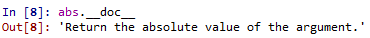
\includegraphics[width=4cm]{figures/kelompok3/1/14.png}
        \centering
        \caption{Hasil Dari abs document}
    \end{figure}
\end{enumerate}
\section{1174026 - Felix Lase}
\subsection{Syntax}
\hfill\break
Python tidak mengadopsi terminator pernyataan, dan blok kode ditentukan melalui
lekukan. Pernyataan yang mengharapkan tingkat indentasi harus diakhiri dengan tanda titik dua (:). Ini mengarah
sebagai berikut:
\begin{itemize}
    \item Kode Python lebih jelas dan lebih mudah dibaca.
    \item Struktur program selalu bertepatan dengan indentasi.
    \item Lekukan yang buruk dapat menyebabkan kesalahan.
\end{itemize}
\lstinputlisting[firstline=9, lastline=13]{src/kelompok3/1/quick.py}

\subsection{Comments}
\hfill\break
Komentar dimulai dengan tanda pagar  dan berada pada satu baris:
\begin{itemize}
    \item  komentar satu baris
\end{itemize}
String multi-baris digunakan untuk komentar multi-baris:
\begin{itemize}
    \item "" "baris pertama dari komentar multi-baris
baris kedua dari komentar multi-baris. "" "
\end{itemize}

\subsection{Assignments}
\hfill\break
Tugas dibuat dengan simbol sama dengan (=). Untuk tes persamaan, jumlah yang sama (==)
digunakan. Anda dapat menambah dan mengurangi nilai menggunakan operator + = dan - =, diikuti oleh
sebuah tambahan. Ini berfungsi dengan banyak jenis data, termasuk string. Anda dapat menetapkan dan
gunakan beberapa variabel pada baris yang sama.
\lstinputlisting[firstline=15, lastline=21]{src/kelompok3/1/quick.py}

\subsection{Data types}
\hfill\break
Struktur paling signifikan dalam Python adalah daftar, tupel, dan kamus. Set telah
diintegrasikan ke dalam Python sejak versi 2.5 (versi sebelumnya tersedia di set
Perpustakaan):
\begin{itemize}
    \item List :Ini mirip dengan array satu dimensi, tetapi Anda dapat membuat daftar itu
mengandung daftar lain.
    \item Dictionaries : Ini adalah array yang berisi pasangan kunci dan nilai-nilai (tabel hash).
    \item Tuples : Ini adalah objek mono-dimensi abadi.
\end{itemize}
\begin{enumerate}
\item List
\lstinputlisting[firstline=24, lastline=30]{src/kelompok3/1/quick.py}
\item Dictionaries
\lstinputlisting[firstline=32, lastline=36]{src/kelompok3/1/quick.py}
\end{enumerate}

\section{npm - nama}
\subsection{kalo perlu}